
\chapter{书面翻译}
\label{chap:translation}
\begin{center}  
  \Large{文档结构相似性算法调研}
\end{center}

\section*{摘要}
  这篇论文对文档结构相似性算法做了简明的调研,包括优化的树编辑距离算法和各种近似
  算法。这些近似算法包括简单加权标签相似度算法,文档结构的傅里叶变换,和将连续序
  列技术应用到结构相似度计算上。我们展示了三个令人惊奇的结果。第一,傅里叶变换的
  方法是所有近似算法中最不精确的一个,同时也是最慢的一个。第二,优化的树编辑距离
  的算法并不一定是最好的用来将不同网站的网页进行聚类的算法。第三,对于许多应用来
  说,最简单的结构的近似可能是最有用也是最有效率的机制。
\section{简介}
随着万维网上大量的文档的出现,自动地处理这些文档,将其应用于信息抽取,近似聚类和
搜索的需求越来越大。在这个领域的主要工作主要集中在文档的内容上。然而,虽然万维网
的继续发展和进化,越来越多的信息被放在结构化的富文本中,从HTML转换到XML。这个结构
化的信息是一个文档意义的重要体现。从文档中辨别出结构上“相似”,或者结构上互
相“包含”的那些文档的方法是一个非常重要那些相关的相似文档关联起来的机制,而这些
文档可能包含不同的文本内容,那些基于文本内容的相似度算法起不到这样的作用。

现在已有几个文档结构在其中起到关键作用的应用。目前的信息提取算法隐式或显式地依赖
文档的结构化元素。结构化的信息能帮助我们将大量的从不同网站上获得的网页整理成一些
可以大致可以比较的集合。这就使得软件能够将可以抽取出正确结果的集合和那些不能抽取
有用信息的集合分离开来。

结构相似度是一个非常重要的话题,有非常多的算法可以计算任意两个文档结构之间的最小
编辑距离。然而,由于这些算法复杂度非常高,通常都需要$O(n^2)$或者更多的时间去计算
距离,因此创造一些更快的,但是距离的计算精确度有些许损失的算法是有可能的。

我们在这篇论文的第二节展示了当前用于检测结构相似度的算法的概述。之后在第三节我们
描述了一个新的基于连续序列的计算结构相似度的近似算法。在第四节我们在速度和精确度
上对比了一下这些近似度算法和优化的树编辑距离算法。在第五节中我们用对不同算法特点
的概括进行了总结。

\section{当前研究状况}
基于树的文档结构性相似度的研究已经有很长的历史了。早期基于树的变换检测来
自[1],[2]。近期Shasha [3], [4], [5]和Chawathe [6],[7]做了一些关于树到树变换的
研究,主要集中在如何创建一个最小的脚本用来进行树之间的转换。在将一些基于结构的相
似度计算修改成半结构的格式方
面也有很多的尝试,包括NiagraCQ [8],Xdiff [9],适用
于XML的Xyleme [10],[11],以及AIDE [12],[13]和适用
于HTML的ChangeDetector\textsuperscript{\texttrademark}。

之前关于HTML文档相似度的工作大部分集中在了内容相似度上,页面分段[15]技术也是一样。
目前的结构相似度集中在了XML的Schema的相似度上。DTD相似度研究集中在对成对的文档和
未知但相似的DTD的近似度计算上。这要求每两篇文档比较一次需要$O(n^2)$的计算复杂度。
其他的工作将文档之间结构相似度的问题转化为用傅里叶变换的时间序列的相似度,实现上
采用快速傅里叶变换以实现$O(n\times lgn)$的复杂度。

在这篇论文中,我们引进了一个将连续序列技术应用在衡量文档结构相似度上的方法。这要
求用$O(k)$的复杂度去创造一个连续序列文档(在这里$k$表示节点的个数),以及提供常数
时间的复杂度进行文档之间的比较。在计算时间上的节省是通过损失计算精确度的得到的,
实际可以任意减小精确度以满足不同的要求。第四节比较了这个技术与其他近似算法在不同
的数据集上的表现。

\subsection{近似算法}
这里我们提供一个对不同类型的用于计算文档相似度算法的概述。我们将描述的衡量标准包
括树编辑距离,标签距离,傅里叶变换和路径相似度。连续序列技术的动机和算法我们将在
第三节给出。

树编辑距离相似度。一些作者提供了一些计算两个树之间优化的树编辑距离的算法。这篇论
文使用Nierman和Jagadish [16]描述的动态编程实现。一般来说,编辑距离衡量的是将一个
树转换为另一个树所要求的插入,删除和更新的最少的节点个数。通过将编辑操作的次数和
较大的那个文档的节点个数之间进行归一化,可以将其转换为相似度的衡量标准。令$N_i$为
文档$D_i$的树形表示的节点集合,于是
\[
TED(D_i,D_j)=\frac{editDistance(D_i,D_j)}{max(|N_i|,|N_j|)}
\]

标签相似度。标签相似度可能是结构相似度最简单的度量方法,因为它只衡量两个标签集合
之间的近似程度。在XML文档中,标签是schema的一个组成部分,使用一个类似标签集合的页
面schema也很有可能类似。两个文档的标签集合可以用来测量它们的重合程度。令$T_i$为
文档$D_i$所包含的标签集合,$T_J$为文档$D_j$包含的标签集合。两个页面的简单的标签
相似度为$T_i$和$T_j$的交集和并集的比例。

然而,由于各种原因,这并不令人满意。一个关键的问题是遵循一个相同schema的页面,比
如HTML,只有一个非常有限的不同标签的个数;一个页面可能包含非常多的一个特殊的标签,
但是用于比较的页面只包含相对很少的这个标签。为了补偿标签频率,我们可以引入一个加
权的相似度度量。令$t_{ik}$为$T_i$的一个成员,$w_{ik}$为标签$t_{ik}$在文档$D_i$中
出现的次数。此外,令$t_{jk}$为$T_j$中对应的标签,$v_{jk}$为$t_{jk}$在文档$D_j$中
出现的次数。如果有$n$个互不相同的标签同时出现在文档$D_i$和$D_j$中,加权标签相似
度可以表示为:
\[
WTS(D_i,D_j)=\frac{\sum_{k=1}^n2*min(w_{ik}, v_{jk})}{\sum_{k=1}^n(w_{ik}+v_{jk})}
\]

由于这个仅包含每个文档中的标签集合,结构相似度的精确性与使用的标签无关。因此,这
个度量方法在类似HTML的环境中应该只有非常低的精确度,这些环境标签集合是很有限的,
但是结构却变化非常大。它在一些都遵循一个小的schema集合的文档上有可能变得更加精确,
因为这些schema限制了文档结构的变化。

傅里叶变换相似度衡量。Flesca \textit{et al.} 引入傅里叶变换作为计算文档相似度的
一个手段。基本的想法是将一个文档的开始标签和结束标签以外的全部信息去掉,只保留一
个表示结构的骨干。然后将这个结构转化为一个数字序列。将这个数字序列视为时序序列,
然后使用傅里叶变换将其转化到频域。最终,两个文档之间的距离可以通过两个信号的幅度
差别进行计算。

这个算法有几个对结果有重大影响的关键组成部分。像一开始所说的,文档结构的编码采用
一个独特的(序列的)正数来表示每一个开始标签,用负数来表示对应的结束标签。属性被
当做标签。注意到这个意味着为了比较两个文档,标签的数字映射必须在每个文档中都是一
样的。Flesca \textit{et al.}选择了一个文档$d$的多层的编码,将其映射成一个序列
$[S_0,S_1,\dots,S_n]$,其中
\[
S_i=\gamma(t_i)\times expF(t_i) + \sum_{t_j\in nest_d(t_i)}\gamma(t_j)\times expF(t_j)
\]
其中$\gamma(t_i)$是一个对应于第$i^{th}$个标签的整数,
$expF(t_i)=B^{maxdepth(D)-l_{t_i}}$是一个决定标签权重的指数因子,$B$是一个固定的
底,$maxdepth(D)$是正在比较的文档的最大深度,$l_{t_i}$是第$i^{th}$个标签的深度,
$nest_d(t_i)$是$t_i$的祖先集合。

最终的两个文档$d_1,d_2$的距离度量通过傅里叶变换定义为
\[
dist(d_1,d_2)=(\sum_{k=1}^{M/2}(|[FFT(h_{1})](k)|-|[FFT(h_2)](k)|)^2)^{\frac{1}{2}}
\]
其中$FFT$傅里叶变换关于同时出现在$h_1$和$h_2$中频率的插值,$h_1$是$d_1$对应的信
号,$M$是出现在插值中的点的个数。

这个方法有一些困难的地方。第一,FFT要求点的个数是2的幂。一个DFT实现使用了和文档的
时序表示一样多的点,意味着DFT和FFT近似算法的精度是不一样的。对于我们的比较而言,
我们发现了FFT当成DFT时是$O(n^2)$的,在实践中它比树编辑距离算法更慢,而且DFT的精
度比FFT的精度要低。

第二,调和标签映射的要求和预先计算用于比较文档的最大深度意味着需要有根据单一文档
来预先计算这个算法的任意部分的能力,以减小成对比较所需的时间。

第三,傅里叶变换典型的用法是在重复的无限时间序列上。我们所碰到的那些文档是有限的。
为了可以使用这个变换,我们必须将从文档中提取的时间序列扩展为无限重复的。对于原始
文档这意味着什么以及这个对于比较有那些影响我们都不清楚。

\section{路径连续序列}
使用优化的树编辑距离算法的问题在于它在大的文档集上代价非常大。目前所展示的近似算
法要么不够直观(傅里叶变换),要么只提供了一个粗略的相似度度量(加权标签算法)。
我们感到需要有一个可以根据应用来调整精度的快速的近似算法。

Shingle是Broder在[15]中为计算文本文件相似度和包含度而引入的技术。这个技术减小了文
档中词或者标记的集合,将其变成一个散列的列表,能够直接和另一个文档进行比较,通过
集合的差集,并集和交集来计算相似度或者包含度。

更进一步地,shingle集合的子集,叫做sketch,可以用于计算文档的相似度。直观地
说,sketch是一个页面的随机采样的一段文本。关键在于由于随机映射在所有的页面中都是
一样的,而且结果是排好序的,这些样本是可以直接在不同的页面之间进行比较。页面采样
的重合度意味着整个页面的重合程度。

我们将展示如何修改这个技术,将其应用到文档的结构中。这使我们可以在线性时间计算文
档结构相似度。通过稍微减小精度,可以实现常数时间的任意大小的文档之间的比较。

\subsection{路径相似度}
为了创建一个适用shingle技术的结构编码,我们必须找出一个方法去创建一个标记的列表,
用于表示这个结构。一些自然的选择,比如使用深度优先或者广度优先的堆编码,因为用于
表示树的标记列表本身的不分段特性从而证明是不合适的。这意味着当一个分支结束和另一
个分支开始的时候,覆盖序列的窗口不能被辨别出来。覆盖这些的窗口不能精确表示原始文
档的任一部分。为了找到用于这种编码的合适的分段方法,衍生了另一个自然的编码方法:
路径。

半结构化的文档(HTML和XML)可以被看成一个由分支和从根到叶的路径组成的序列。为了我
们的目标,我们将任意的部分路径,即从根到文档中任意的节点组成的路径也认为是一个标
记。一个树可以用一个这些标记的序列来表示。比如,HTML中最简单的树有一个title和
body元素,可以被编码为:\\
/html\\
/html/head\\
/html/head/title/\\
/html/head/title/[text]\\
/html/body
/html/body/[text]

路径相似度衡量两个不同文档之间的路径的相似度。一个路径被定义为一个从根节点开始,
到叶子节点结束的相连的节点列表。路径相似度可以从多种方式进行度量:二元的,路径要
么相等或者不相等;部分的,在每个路径中可以比较的节点的数目是知道的;或者加权的,
节点根据它到根的距离进行加权。

部分路径相似度需要很大的计算代价。因为两个树的路径有$n!$种可能的映射,用穷举的算
法来产生优化的相似度分数是不可行的。二元的相似度代价要小很多,因为在一个版本中的
每一个独特的路径可以通过数据库的join技术来匹配另一个版本中的等价路径。相似度可以
通过匹配上的路径个数和两个树总的路径数的比例来计算。

\subsection{将shingle应用到路径上}
一个shingle是一个从文档中得到的连续的标记的子序列。两个文档的相似性定义为
\[
r(D_i,D_j)=\frac{S(D_i,w)\cap S(D_j,w)}{S(D_i,w)\cup S(D_j,w)}
\]
然而$S(D_i,w)$是从文档$D_i$创建长度为$w$的shingle的操作符。类似地,文
档$D_i$和$D_j$的包含度定义为
\[
c(D_i,D_j)=\frac{S(D_i,w)\cap S(D_j,w)}{S(D_i,w)}
\]

为了方便和快速的处理,shingle可能通过散列函数转换成数字。这个散列函数应该有较高的
可信度使得两个shingle散列成一个数的冲突的可能性变得很小。让散列的空间显著大
于shingle的空间可以使得构造这样一个合适的散列函数变得容易很多。依据一个shingle中
标记的个数(或者窗口的长度),这可能会非常微妙。

一个将结构化比较的复杂度减小到$O(1)$的关键技术是每个文档只保留一个相对小的sketch。
从[15]中我们可以看到从一个shingle集合的排列中进行随机采样得到的样本可以被当成两
个文档之间相似度的无偏估算子。一个有效的实现这个的办法是通过伪随机数生成算法来散
列值,将结果排序,然后选择最小的$k$的结果。

为了将shingle应用到路径结构中,我们定义$S(D_i,w)$如下:对于$D_i$的树形表示中的每
个节点,计算从根到该节点的路径;根据这个(部分)路径的标签名列表创建一个散列;将
该散列加入到当前窗口;窗口向前滑动一个单位(即将窗口的第一个散列值去掉)。。

注意到根据定义,shingle集合可能是一个集合或是一个包——类似于标签相似度和加权标签相
似度之间的差别。于是就出现了使用一个集合来包含shingle会显著减小shingle的表达能力,
并将更大的误差引入到估计中。

我们测量了路径shingle和部分路径shingle的精度。比较是在使用无穷的$k$的不同的窗口大
小下进行的。用来比较是数据是从\texttt{my.yahoo.com}下载的在两年时间内的典型的网页
快照。结果显示小的窗口大小(从1到4)对精度没有影响:两个聚类都没有错误,四个聚类
只引入百分之三的错误。用来比较的shingle个数的不同并不影响聚类的效果。$k$的值从10
测试到了1000,以及一个无穷数量的shingle。所有的都显示了错误在百分之十之内。

\section{实验}
在这一节中我们经验性地评价不同的近似算法与树编辑距离相比的精度,同时还比较了不同
的近似算法的性能。

所有的实验都是在一个配置了速龙双核2G赫兹的处理器,2.4Linux内核的工作站上运行。算
法使用Java实现的,在Sun 1.4.2 JVM上执行。所有的算法都采用了页摘要数据结构来实现,
该数据结果比DOM树表示有很大的性能提升。性能的测量是取10次运行的平均值。

根据聚类进行比较。聚类是在树编辑距离的基础上用来衡量不同度量之间的效果的。树编辑
距离是可证明的一个两个树之间的最佳的编辑距离。我们假定这是最好的相似度度量。其他
的算法会产生一些不同的距离度量,不能直接和一个编辑距离进行比较。然而,如果一个大
的文档集合是根据某个度量方法来聚类的,这些通过不同的度量方法产生的聚类是可以通过
给定同一个聚类方法进行比较的。换句话说,如果两个文档通过树编辑距离判断是相似的,
那么其他的度量也应该认为这两个文档是相似的,或者恰恰相反。

我们可以将一个在一个近似算法中被放在一个shingle聚类中,而在树编辑距离算法中放到
另一个类中的归类成错误文档。这个错误度量有一些缺点。比如,一个文档集合被分成两个
聚类,任何度量都会有严格小于50\%的最大错误率。一般地,随着聚类数目$n$的增长,最
大错误率严格小于$1-\frac{1}{n}$。

我们用两个数据集进行聚类。第一个是从500个XML文档中综合生成的集合。这个集合建模一
个书仓库,每个文档都列出一个书对应的作者,发行商和发行时期。文档之间唯一的结构差
别在于这本书的作者的个数。

每个度量方法都用来度量两个文本之间距离。文档根据这些距离通过开$k-means$进行聚类。
通过每种度量得到的聚类与树编辑距离得到的聚类进行比较,计算一个错误估计。结果显示
在Table I中。
{\centering
  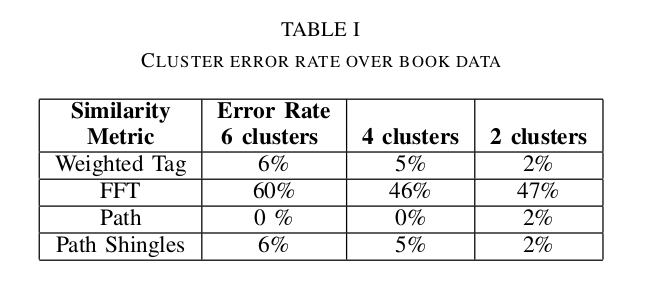
\includegraphics[width=\textwidth]{translationTable1}
}
我们测试了最多6个聚类,因为这个数据集中根据书籍的作者数量,有6个自然的聚类。我们
期望加权标签度量有较低的错误率,因为这些数据之间的结构差异只有\texttt{author}这
个标签出现的次数。

第二个数据集是一系列从以下网站得到的快照:\texttt{cnn.com},
\texttt{corona.bc.ca},\texttt{news.gnome.org},\texttt{10-10phonerates.com}和
\texttt{my.yahoo.com}。快照是2001到2003两年期间的,大概是每天一次。冗余的快照
(由MD5签名决定)被移除了,每个站点的快照集合取样20份页面。一样的聚类算法用在这
些文档上,只有这次我们有一个预定义好的聚类(通过网站),并且可以将每个算法同这些
预定义好的聚类进行比较。结果显示在Table II中。
{\centering
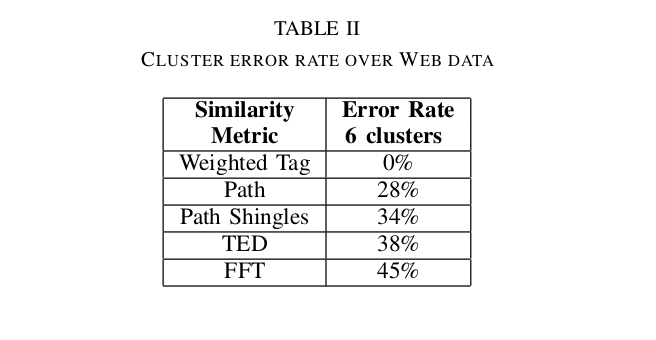
\includegraphics[width=\textwidth]{translationTable2}
}

这个错误率好像异常地高,特别是对于我们在其他测试中用来当做基准的树编辑距离算法。
我们推测这个错误率是由于HTML的结构中用来呈现给用户内容的词汇相对较小。路径和路
径shingle度量比树编辑距离性能要好,但也比预期的要差。这可能是因为它们使用了部分路
径来描述树的结构。很深的树在顶部区域可能会呈现很多相似的结构,导致两个来自不同站
点的树的相似度可能会互相偏向。FFT度量方法的糟糕的性能不能给出一个简单的解释。可以
说依据相同的最开始的一批标签(\texttt{html},\texttt{head}和\texttt{body}),每个
网页都是极度相似的信号,在叶子层面也是相似的构造(标签列表和文本)。然而,这个转
换使得我们难以找出是网页的哪一些特征导致它们变得如此相似。

作为最后的比较,我们检查了以上表格中从一个站点来的快照。这会在比如监测一个页面随
着时间变化的时候很有用。我们选择\texttt{my.yahoo.com}因为里面的内容会定期发生变
化,但是结构上随着时间的变化很缓慢(比如,当一个新的图片被加入到一些特点的假日)。
我们再次把使用近似算法和树编辑距离产生的聚类进行比较。
{\centering
  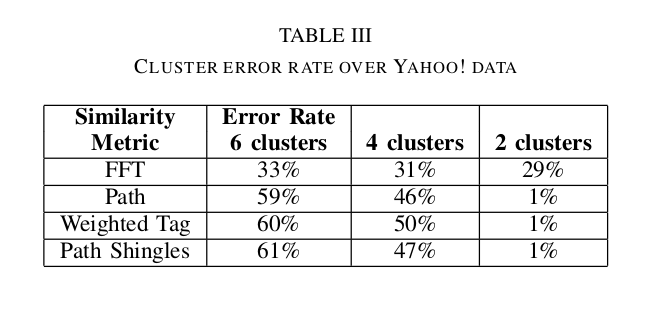
\includegraphics[width=\textwidth]{translationTable3}
}

我们观察到除了FFT以外的大部分近似算法在小的聚类大小上都有非常低的错误率,但是错误
率在聚类的规模变大时会激增。观察一下描述树编辑距离聚类和FFT聚类以及路径/路径
shingle聚类之间映射变化的矩阵是有意义的。Table IV描述了FFT聚类和树编辑距离聚类的
不同,Table V描述了路径聚类和树编辑距离聚类之间的不同。
{\centering
  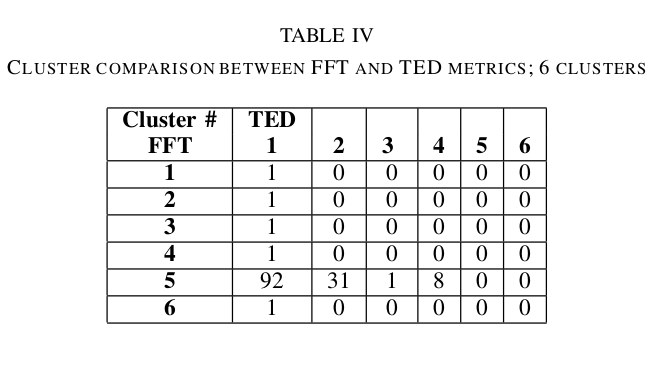
\includegraphics[width=\textwidth]{translationTable4}
}

从这两个矩阵我们可以推导出FFT度量会倾向于将所有的数据点聚成一个类别,因此不提供一
个有效的分辨相似网页的能力。在另一方面,路径度量(路径shingle和加权标签度量实际是
一样的)比树编辑距离更有分辨能力,能够比树编辑距离分出更好的类别。尽管这些实验中
将这种情况标为了错误,它可能有很重要的分辨那些感觉上不一样,但在相同的编辑距离内
的树的功能。

最惊奇的观察在于加权标签的相似度度量方法,一开始我们认为是一文不值的东西,却能和
复杂很多的技术达到一样的精确程度。这可能可以归因为大部分实验是在来自一个站点的相
对同构的页面上进行的(就像书籍数据集或者Yahoo!数据集的情况一样),或者可以归因为
非同构的站点为了突出它们的对比而使用了不同HTML标签子集。另一个观察是傅里叶变换技
术在很简单的数据集上表现也很差。这就使得我们认为尽管这是一个将结构转换为一个更简
单的用于比较的格式的想法,但是它并不适用与文档结构,无论是从分析上还是实验上。

\subsection{性能比较}
选择一个近似算法的主要原因是为了将速度提高到一个可以接受的水平,因为最优的算法太
慢了。文档聚类用于数据抽取或者搜索和获取方法,提供了一个结构化相似度的很好的例
子。用于精度估计的相对小的数据集说明了近似算法在计算近似相似度上的有效性。Figure
1展示了不同算法在书籍文档的数量对数增长时的相对代价。

聚类的时间是在一个小于一千比特的较小的文档上计算的。为了更好地理解计算两个文档之
间差异的代价,我们比较了在TCP-H基准测试数据上的每个度量方法的代价。这个数据是
由Toxgene [19]XML文档生成器随机生成的。我们修改了生成器的参数以便产生包含原始数据
集合1\%,5\%,10\%,15\%,20\%,和25\%的文档。这个生成器跑两次,在每个分数上产生
两个不同的文档。结果在Figure 2中。

我们可以看到树编辑距离算法比任何其他的近似算法都要慢好几个数量级。FFT算法也显示
出了尽管它用很大的精度换来了速度,它仍然比加权标签或者路径shingle方法慢一个数量
级,后两者的精度还显著更高。

大文件支持。以空间换时间的优化对于小到中型大小的文件都工作地很好,但是树编辑距离
在其数据结构会超过物理内存的大文件上明显变慢。当物理内存被耗尽,机器被迫开始使用
交换内存——这个会慢好几个数量级。

shingle在创建常数大小的大文件指纹时有优势,消除了在计算时在内存中维护复杂数据结构
的需要。

shingle还可以部分调优,就算是因此取了原始的指纹。给定一个窗口散列的集合,只有最前
面的$k$个需要比较。用于比较的散列的数目可以调整,把精度用来换速度和空间。这就使得
对于更低精度的比较,一次性可以有更多的指纹在内存中驻留。

\section{总结}
我们展示了一些测量文档结构相似度的算法,比较了它们的精度和性能。我们有了一些有趣
的发现。

第一,我们提供了一个对[17]中所描述的傅里叶变换的实验性的批判。尽管相比最优化树编
辑距离算法,傅里叶变换方法是一个更快的方法,但这个方法没有提供在不同情境中的一个
精确的相似度衡量。此外,这个技术的性能也通常比其他更直观的相似度计算方法要差。

第二,对于很多结构相似度的应用来说,最简单的计算标签数量的方法提供了最好的性能情
况下的一个可以接受的精度。我们一开始将加权标签相似度当成一个不重要的计算结构相似
度最快的近似方法。然而,结果是它可以和其他任何近似算法表现一样好,甚至更好。尽管
它没有像树编辑距离方法一样(匹配的相同子树),或者路径shingle方法一样(子结构包含
性)提供一定的结构特征,但是对于不需要这些特征的应用来说,这个算法既快又有辨别
力。

最后,我们基于文档结构中的路径展示了一个新的相似度度量。我们通过应用shingle技术,
可以从任意的文档中创建常数大小的表示方法,使得比起其他相似度度量,聚类方法可以应
用到大很多的文档集合中。此外,这种度量具有在一个大文档集合中搜索子结构和在基于树
的文档集合中做一些结构化的挖掘的能力。

\section*{致谢}
作者要感谢Chunk Baldwin和Ghaleb Abdulla,他们刺激了这些话题之间的对话。作者还要感
觉Daniel Rocco,他搭建了第一个实验框架,并帮助开发了页面摘要数据结构,作为许多算
法的基础。

这个工作是基于No. W-7405- ENG-48. UCRL-CONF-202728法令,在美国能源部的保护下,
在University of California Lawrence Livermore National Laboratory进行的,

\section*{参考文献}
\begin{enumerate}[{[}1{]}]
\item K. C. Tai, “The tree-to-tree correction problem,” Journal of the ACM,
  vol. 26, no. 3, 1979.
\item S. Y. Lu, “A tree-to-tree distance and its application to cluster
  analysis,” IEEE Trans. Pattern Anal. Mach. Intell. PAMI-1, no. 2, 1979.
\item D. Shasha and K. Zhang, “Fast algorithms for the unit cost editing
  distance between trees,” Journal of Algorithms, no. 11, 1990.
\item K. Zhang, D. Shasha, and J. T.-L. Wang, “Approximate tree matching in the
  presence of variable length don’t cares,” J. Algorithms, vol. 16, no. 1, pp.
  33–66, 1994. [Online]. Available: citeseer.nj.nec.com/zhang93approximate.html
\item D. Shasha and K. Zhang, “Approximate tree pattern matching,” in Pattern
  Matching Algorithms. Oxford University Press, 1997, pp. 341–371. [Online].
  Available: citeseer.nj.nec.com/95609.html
\item S. Chawathe, A. Rajaraman, H. Garcia-Molina, and J. Widom, “Change
  detection in hierarchically structured information,” in Proceedings of ACM
  SIGMOD, 1996.
\item S. S. Chawathe and H. Garcia-Molina, “Meaningful change detection in
  structured data,” in Proceedings of the 1997 ACM SIGMOD, 1997, pp. 26–37.
  [Online]. Available: citeseer.nj.nec.com/article/chawathe97meaningful.html
\item J. Chen, D. DeWitt, F. Tian, and Y. Wang, “NiagaraCQ: A scalable
  continuous query system for Internet databases,” in Proceedings of the 2000
  ACM SIGMOD, 2000.
\item Y. Wang, D. DeWitt, and J.-Y. Cai, “X-Diff: An effective change detection
  algorithm for XML documents,” International Conference on Data Engineering,
  2003.
\item A. Marian, S. Abiteboul, G. Cobena, and L. Mignet, “Change- centric
  management of versions in an XML warehouse,” in The VLDB Journal, 2001, pp.
  581–590. [Online]. Available: citeseer.nj.nec.com/marian00changecentric.html
\item G. Cobena, S. Abiteboul, and A. Marian, “Detecting changes in XML
  documents,” in International Conference on Data Engineering, 2002, pp. 41
  –52.
\item F. Douglis, T. Ball, Y.-F. Chen, and E. Koutsofios, “The AT\&T Internet
  difference engine: Tracking and viewing changes on the Web,” in World Wide
  Web, vol. 1, January 1998, pp. 27–44.
\item Y.-F. Chen, F. Douglis, H. Huan, and K.-P. Vo, “TopBlend: An efficient
  implementation of HtmlDiff in Java,” in Proceedings of the WebNet2000
  Conference, San Antonio, TX, November 2000.
\item V. Boyapati, K. Chevrier, A. Finkel, N. Glance, T. Pierce, R. Stokton, and
  C. Whitmer, “ChangeDetector(TM): A site-level monitoring tool for the WWW,”
  in WWW2002, May 2002.
\item A. Z. Broder, “On the Resemblance and Containment of Documents,” in
  Proceedings of Compression and Complexity of SEQUENCES 1997, 1997.
\item A. Nierman and H. Jagadish, “Evaluating structural similarity in XML
  documents,” Fifth International Workshop on the Web and Databases, 2002.
\item S. Flesca, G. Manco, E. Masciari, L. Pontieri, and A. Pugliese, “Detect-
  ing structural similarities between XML documents,” Fifth International
  Workshop on the Web and Databases, 2002.
\item D. Rocco, D. Buttler, and L. Liu, “Page Digest for large-scale Web ser-
  vices,” in Proceedings of the IEEE Conference on Electronic Commerce, June
  2003.
\item D. Barbosa, A. O. Mendelzon, J. Keenleyside, and K. A. Lyons, “Toxgene:
  An extensible template-based data generator for XML,” in SIGMOD Conference,
  2002. [Online]. Available: citeseer.nj.nec.com/525958.html
\end{enumerate}
%%% Local Variables: 
%%% mode: latex
%%% TeX-master: "../main"
%%% End: 
